%----------------------------------------------------------------------------
\chapter{Megvalósítás}\label{sect:megvalositas}
%----------------------------------------------------------------------------

A megvalósítás során csak az \textbf{objektumorientált programozás} (object-oriented programming -- OOP) merült fel mint felhasználható módszertan. Az általánosan elterjedt koncepció lehetővé teszi egy komplex probléma kellően intuitív megfogalmazását és átlátható leírását. Erre a fejlesztés során szükség is volt, hiszen a meglehetősen összetetté váló programot csak gondos tervezéssel és kivitelezéssel lehetett megfelelő minőségben előállítani.

Az alkalmazás fejlesztését tehát az OOP paradigmáinak szem előtt tartásával végeztem. Az ismert alapelvek néhány szóban:

\begin{itemize}
  \item \textbf{absztrakció (abstraction):} a probléma valós világbeli objektumok mintájára történő modellezése, a lényegtelen részletek elhagyásával, a lényeges tulajdonságok kiemelésével
  \item \textbf{egységbe zárás (encapsulation):} az egyes osztályok és objektumpéldányok saját maguk rendelkezzenek a futások során szükséges adatok és metódusok felett
  \item \textbf{öröklődés (inheritance):} lehetséges egy általános ősosztály tetszőleges kiegészítése, specializálása a közös elemek megtartásával
  \item \textbf{polimorfizmus (polymorphism):} az egyes műveleteket képesek legyünk bemeneti paraméterek széles skáláján végrehajtani (metódus- vagy operátor-felüldefiniálás)
\end{itemize}

\bigskip

\texttt{+++ melyik szakaszban mi van +++}

%,,,,,,,,,,,,,,,,,,,,,,,,,,,,,,,,,,,,,,,,,,,,,,,,,,,,,,,,,,,,,,,,,,,,,,,,,,,,
\section{Követelmények}\label{sect:kovetelmenyek}
%,,,,,,,,,,,,,,,,,,,,,,,,,,,,,,,,,,,,,,,,,,,,,,,,,,,,,,,,,,,,,,,,,,,,,,,,,,,,

Mielőtt a fejezet későbbi szakaszaiban részletekbe menőben bemutatom az elkészült alkalmazás architektúráját, illetve osztályainak pontos működését, szeretném dokumentálni a kész programra vonatkozó \textbf{követelményeket, azaz specifikációt}.

\bigskip

Az alkalmazás legyen képes:

\begin{enumerate}[a)]
  \item valósidejű \textbf{videofolyamot} olvasni a számítógépre kötött webkameráról (lásd \sectref{infracam} szakasz)
  \item a videofolyam feldolgozásával a \textbf{pupillapozíció meghatározására} a \sectref{pupillakov} szakaszban leírtak szerint.
  \item a tekintet \textbf{kalibrációjára} a \sectref{kalibracio} szakaszban ismertetett módszer felhasználásával.
  \item \textbf{munkamenetek} (session) rögzítésére a képernyő tartalmának mentésével együtt.
  \item a korábbi munkamenetek listázására, törlésére.
  \item munkamenetek \textbf{visszajátszására}.
  \item a munkamenetek alapján \textbf{hőtérképek} generálására (lásd \sectref{web} szakasz)
\end{enumerate}

%,,,,,,,,,,,,,,,,,,,,,,,,,,,,,,,,,,,,,,,,,,,,,,,,,,,,,,,,,,,,,,,,,,,,,,,,,,,,
\section{Architektúra}\label{sect:architektura}
%,,,,,,,,,,,,,,,,,,,,,,,,,,,,,,,,,,,,,,,,,,,,,,,,,,,,,,,,,,,,,,,,,,,,,,,,,,,,
  
  Az implementációt a \sectref{technologia} fejezetben bemutatott technológiák (OpenCV, Qt, Qt Creator) felhasználásával \textbf{C++ nyelven készítettem el} a Model--View--Controller (MVC) tervezési minta szem előtt tartásával. A kialakított osztályhierarchia a \figref{overview} ábrán látható módon épül fel. A kibővített osztálydiagram  -- a fontos változók és funkciók feltüntetésével -- megtalálható az \sectref{osztalydiagram} függelékben.

\begin{figure}[!ht]
\centering
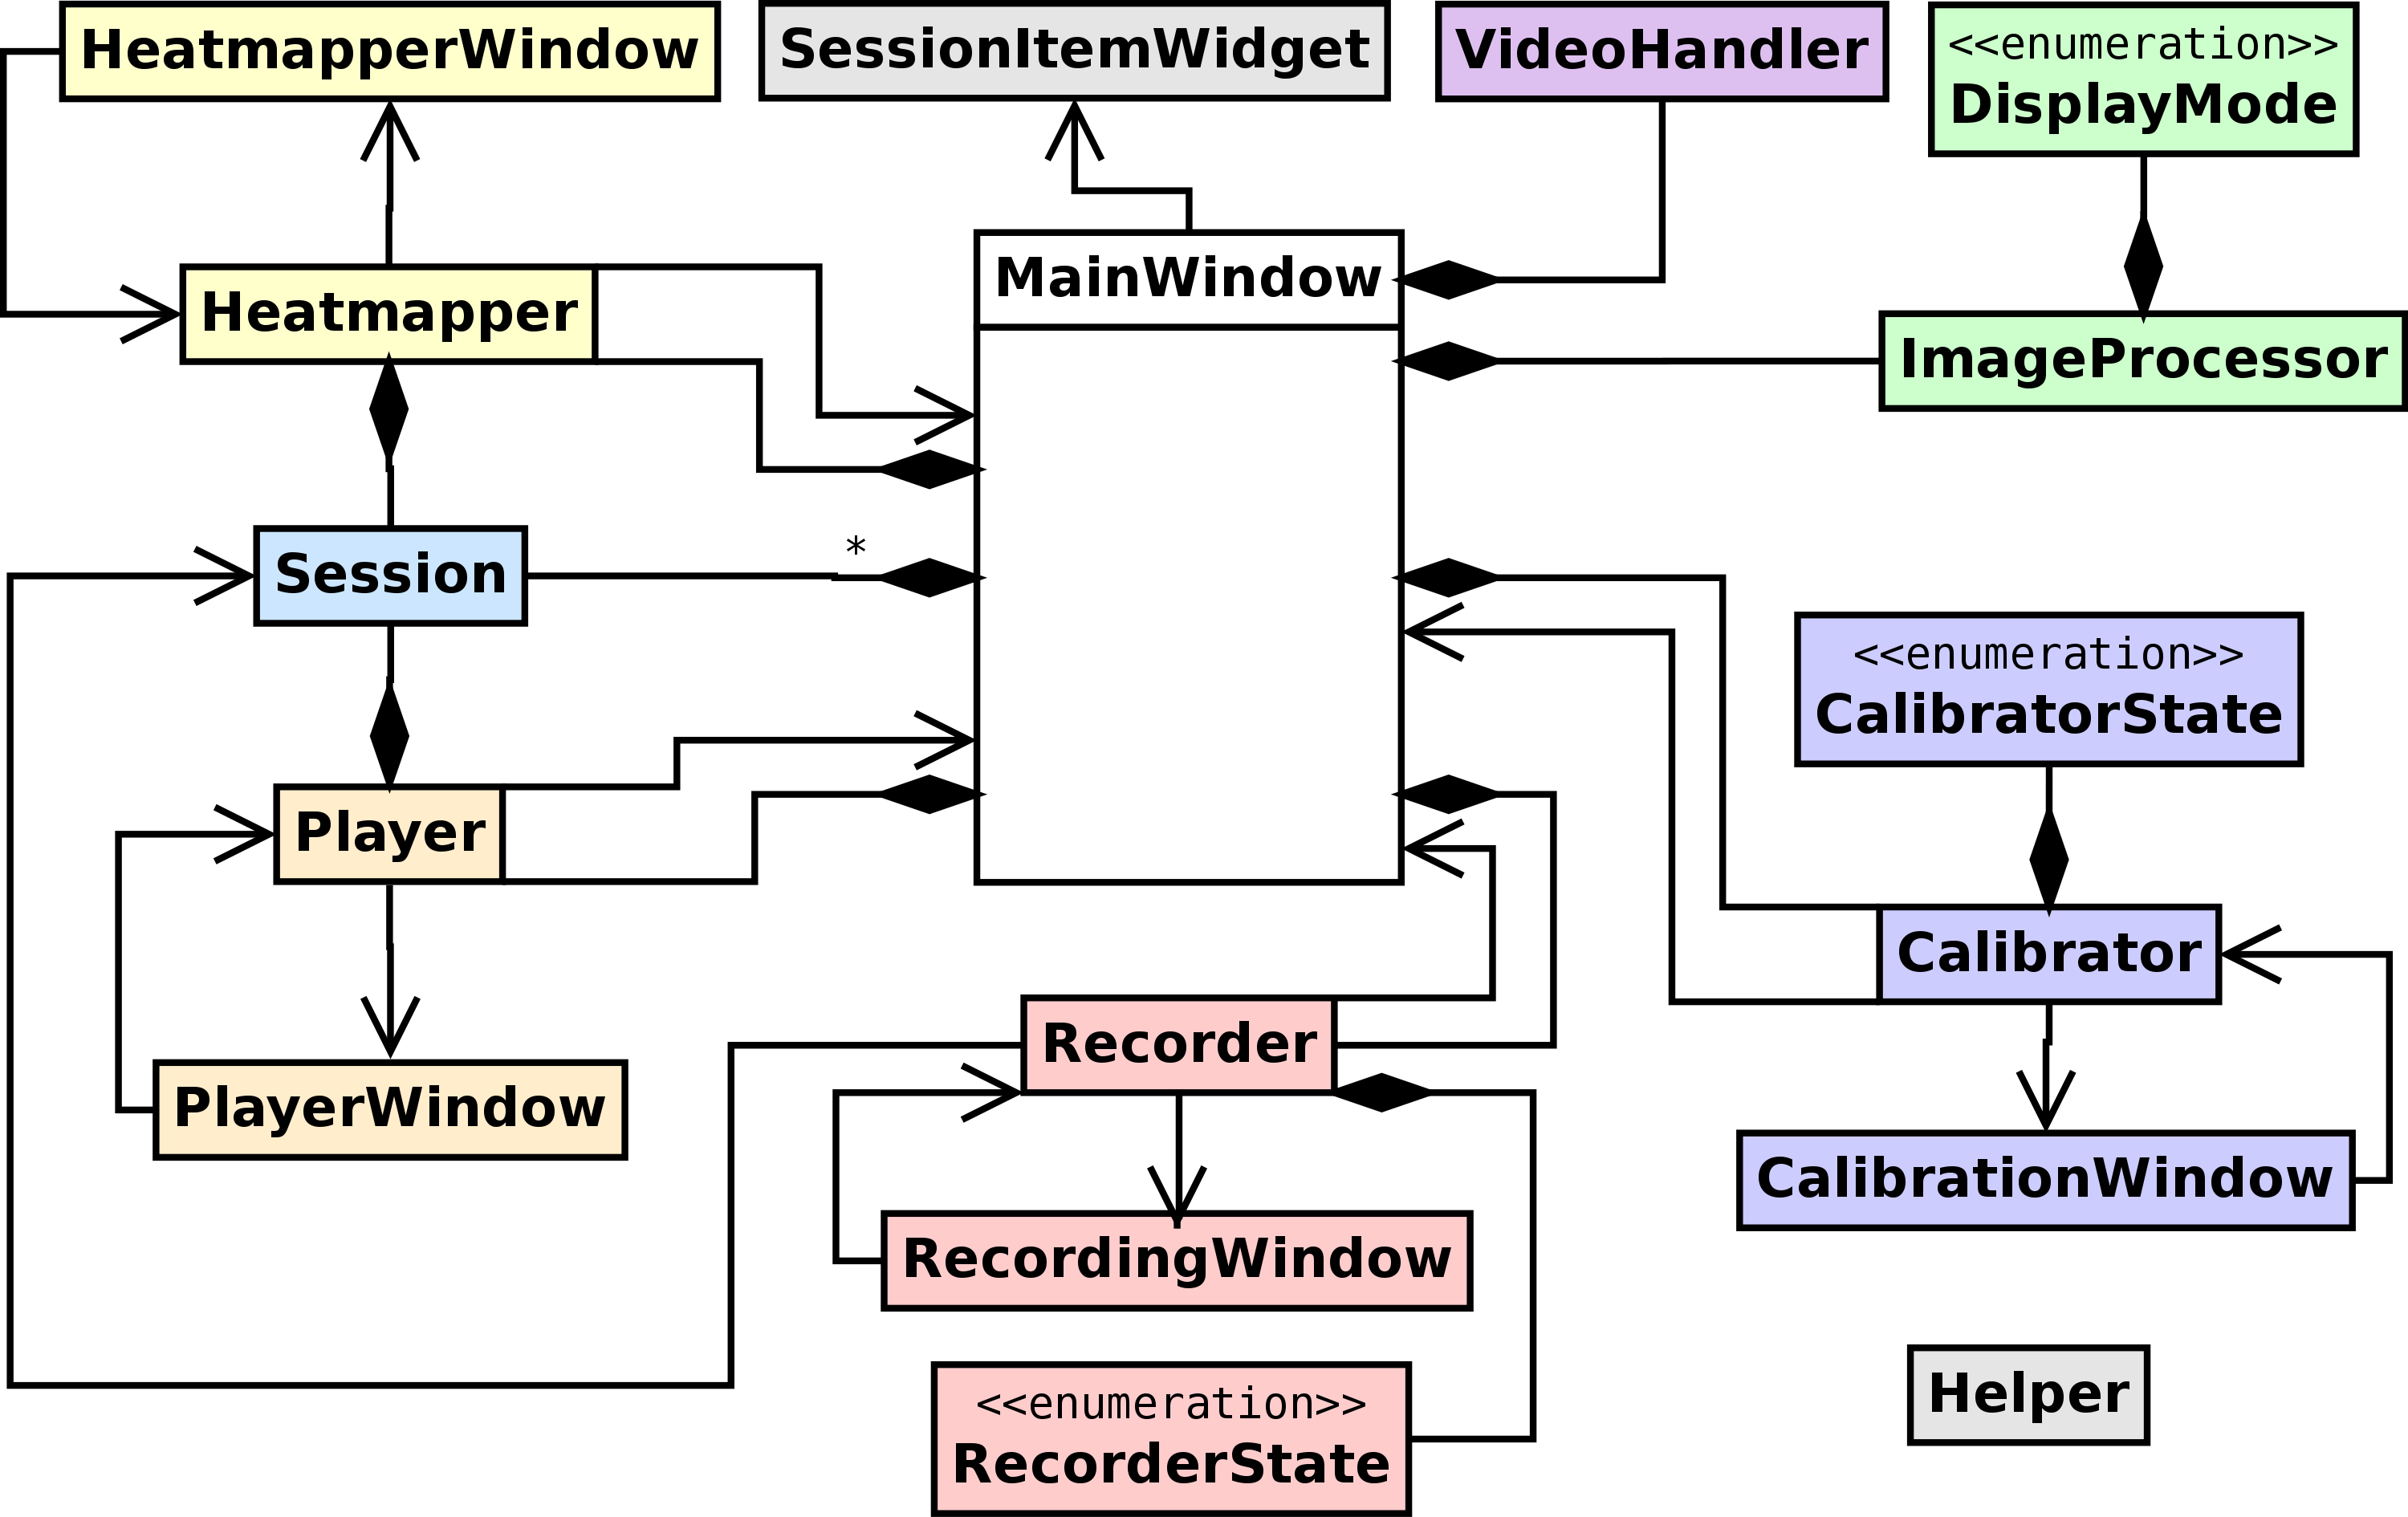
\includegraphics[width=140mm, keepaspectratio]{figures/overview_aa.png}
\caption{Az alkalmazás osztályhierarchiája}
\label{fig:overview}
\end{figure}

Az alkalmazás egyes funkcióit a videofolyam feldolgozásától egészen a hőtérképek generálásáig osztályok egy-egy csoportja végzi. A \figref{overview} ábrán színkódokkal jelöltem a logikailag összetartozó osztályokat. A specifikáció egyes pontjait kielégítő osztályok az ábráról leolvasva, felsorolás szintjén:

\begin{itemize}
  \item \texttt{MainWindow} -- az alkalmazás főablakát tartalmazó osztály, valamint ez szolgál általános kontrollerként is, lévén a felhasználói interakciók döntő része ide fut be
  \item \texttt{VideoHandler} -- a webkameráról beérkező videofolyam olvasásáért felelős
  \item \texttt{ImageProcessor} -- a képkockák feldolgozását -- a pupillakeresést -- végzi
  \item \texttt{Calibrator} -- a kalibrációt, majd kalibrált állapotban a \emph{pupilla-pozíció} $\Longrightarrow$ \emph{képernyő-pozíció} átszámítást végzi
  \item \texttt{Recorder} -- a munkamenetek rögzítését végzi
  \item \texttt{Player} -- a felvett munkamenetek visszajátszását teszi lehetővé ez az osztály
  \item \texttt{Heatmapper} -- a hőtérképek generálása történik ebben az osztályban
  \item \texttt{Session} -- konténerosztály egy-egy munkamenet futásidejű tárolása számára 
\end{itemize}

A továbbiakban sorra veszem az egyes osztályok interfészét, valamint belső működésüket, kicsit mélyebb betekintést engedve a felépítésükbe, egymással való összeköttetésükbe, valamint az esetleg érdekesnek ítélhető implementációs részletekbe.

%............................................................................
\subsection{A \texttt{MainWindow} osztály}\label{sect:mainwindow}
%............................................................................

\begin{figure}[!ht]
\centering
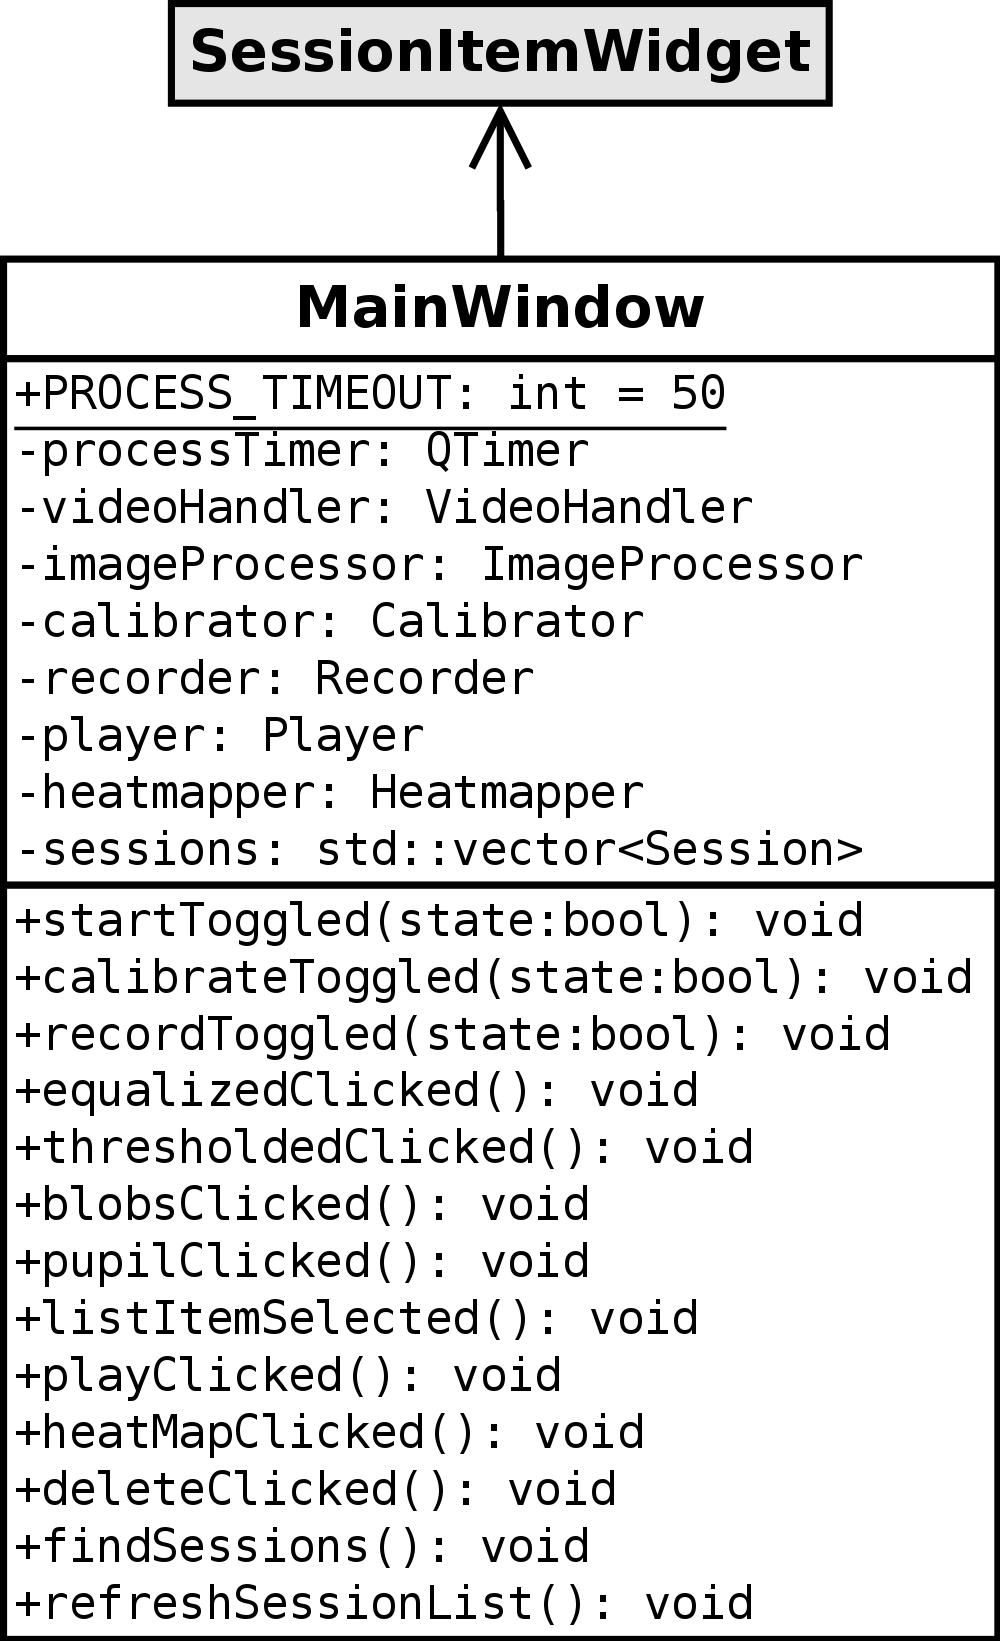
\includegraphics[width=50mm, keepaspectratio]{figures/class_mainwindow.png}
\end{figure}

A \texttt{MainWindow} osztály az alkalmazás általános kontrollereként működik. A nevéből is látszik, hogy ehhez az osztályhoz tartozik a program fő interfészablaka, ennek megfelelően a felhasználói interakciók lekezelése ezen osztály slotjaiban történik. Az osztályban tényleges feldolgozás nem történik, csak összefogja az egyes lépéseket elvégezni hivatott objektumokat.

\bigskip

Az \texttt{int PROCESS\_TIMEOUT} attribútum a \texttt{QTimer processTimer} időzítővel együtt a feldolgozás rögzített sebességgel történő elvégzését vezérli. Az előbbi ezredmásodpercben megadott értéke alapján hívódik a feldolgozást vezérlő \texttt{processTimeout()} függvény.

A \texttt{sessions} lista az elmentett munkamenetek futásidejű tárolására szolgál, amely listát a \texttt{refreshSessionList()} függvény állítja elő.

A \texttt{videoHandler}, \texttt{imageProcessor}, \texttt{calibrator}, \texttt{recorder}, \texttt{player} és \texttt{heatmapper} attribútumok tárolják a névből adódó típusú objektumpéldányokat, amelyek az alkalmazás egyes funkcióit valósítják meg.

A metódusok közül a \texttt{startToggled()}, \texttt{calibrateToggled()} és \texttt{recordToggled()} metódusok sorra a videofolyam, kalibráció és a felvétel ki/bekapcsolását kezelik le.

A lejátszás során megjelenítési módok váltását kezelik le az \texttt{equalizedClicked()} és a \texttt{pupilClicked()} között felsorolt függvények.

%............................................................................
\subsection{A \texttt{VideoHandler} osztály}\label{sect:videohandler}
%............................................................................

\begin{figure}[!ht]
\centering
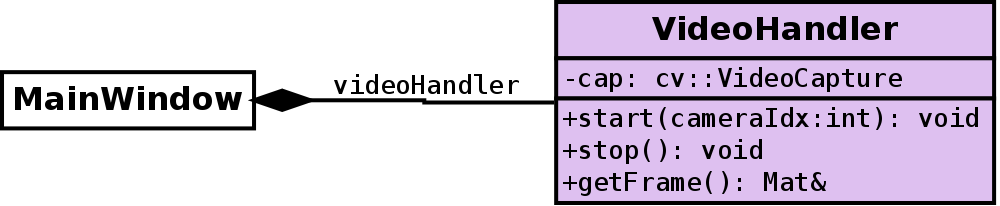
\includegraphics[width=100mm, keepaspectratio]{figures/class_videohandler.png}
\end{figure}

blabla

%............................................................................
\subsection{Az \texttt{ImageProcessor} osztály}\label{sect:imageprocessor}
%............................................................................

\begin{figure}[!ht]
\centering
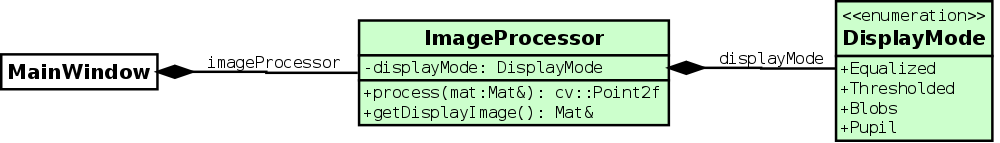
\includegraphics[width=100mm, keepaspectratio]{figures/class_imageprocessor.png}
\end{figure}

blabla

%............................................................................
\subsection{A \texttt{Calibrator} osztály}\label{sect:calibrator}
%............................................................................

\begin{figure}[!ht]
\centering
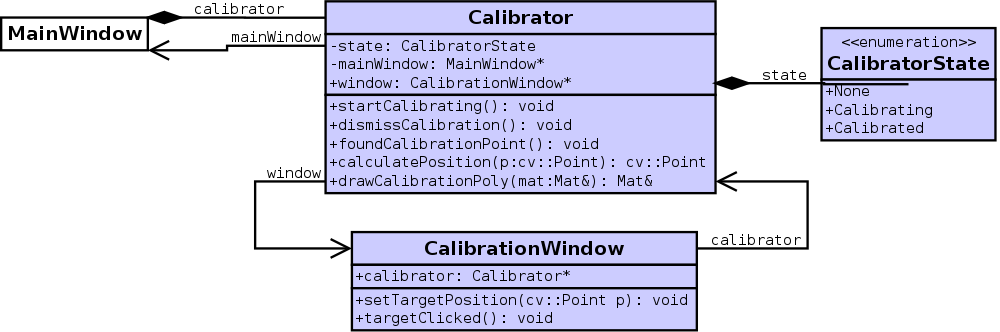
\includegraphics[width=100mm, keepaspectratio]{figures/class_calibrator.png}
\end{figure}

blabla

%............................................................................
\subsection{A \texttt{Session} osztály}\label{sect:session}
%............................................................................

\begin{figure}[!ht]
\centering
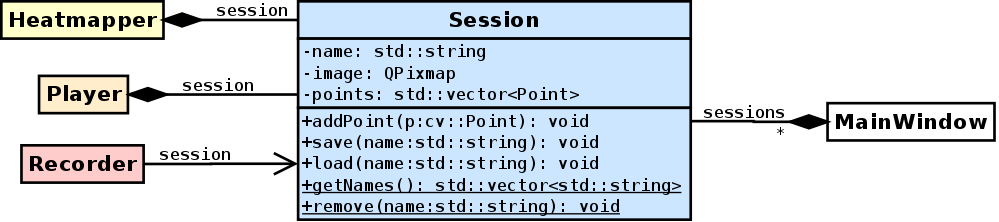
\includegraphics[width=100mm, keepaspectratio]{figures/class_session.png}
\end{figure}

blabla

%............................................................................
\subsection{A \texttt{Recorder} osztály}\label{sect:recorder}
%............................................................................

\begin{figure}[!ht]
\centering
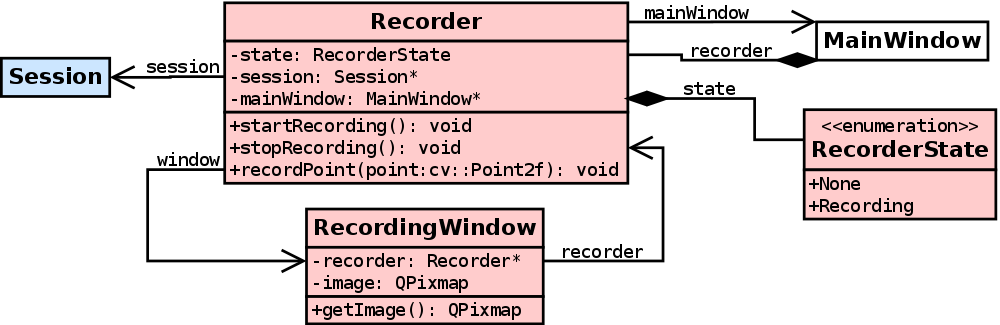
\includegraphics[width=100mm, keepaspectratio]{figures/class_recorder.png}
\end{figure}

blabla

%............................................................................
\subsection{A \texttt{Player} osztály}\label{sect:player}
%............................................................................

\begin{figure}[!ht]
\centering
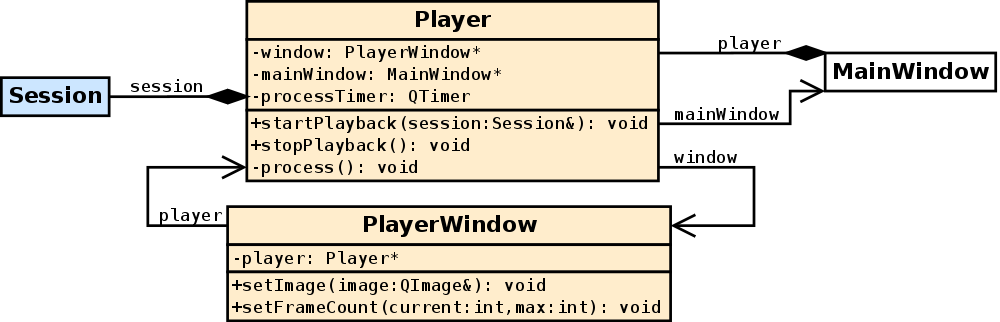
\includegraphics[width=100mm, keepaspectratio]{figures/class_player.png}
\end{figure}

blabla

%............................................................................
\subsection{A \texttt{Heatmapper} osztály}\label{sect:heatmapper}
%............................................................................

\begin{figure}[!ht]
\centering
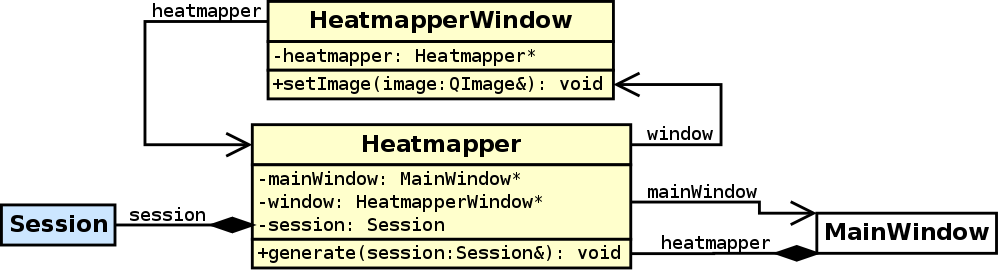
\includegraphics[width=100mm, keepaspectratio]{figures/class_heatmapper.png}
\end{figure}

blabla

%,,,,,,,,,,,,,,,,,,,,,,,,,,,,,,,,,,,,,,,,,,,,,,,,,,,,,,,,,,,,,,,,,,,,,,,,,,,,
\section{Felhasználói felület}\label{sect:gui}
%,,,,,,,,,,,,,,,,,,,,,,,,,,,,,,,,,,,,,,,,,,,,,,,,,,,,,,,,,,,,,,,,,,,,,,,,,,,,

\texttt{+++ leiras + kepek a felhasznalo feluletrol +++}

%,,,,,,,,,,,,,,,,,,,,,,,,,,,,,,,,,,,,,,,,,,,,,,,,,,,,,,,,,,,,,,,,,,,,,,,,,,,,
\section{Felhasználói dokumentáció}\label{sect:docs}
%,,,,,,,,,,,,,,,,,,,,,,,,,,,,,,,,,,,,,,,,,,,,,,,,,,,,,,,,,,,,,,,,,,,,,,,,,,,,

\texttt{+++ az alkalmazas pontos hasznalata (tobb monitor, stb) +++}

%,,,,,,,,,,,,,,,,,,,,,,,,,,,,,,,,,,,,,,,,,,,,,,,,,,,,,,,,,,,,,,,,,,,,,,,,,,,,
\section{Tesztelés, eredmények}\label{sect:teszteles}
%,,,,,,,,,,,,,,,,,,,,,,,,,,,,,,,,,,,,,,,,,,,,,,,,,,,,,,,,,,,,,,,,,,,,,,,,,,,,

\texttt{+++ tesztelesi dokumentacio (ide mit?) +++}